
\chapter{Background}
\todo{
 
\section{Discrete Timme Event Systems}
\label{sec:discreteEventTimeSystems}

\subsection{Petri Nets}
\label{sec:petriNets}

\subsubsection{Control Interpreted Petri Net}

\subsection{Automata}
\label{sec:automata}

\section{Model of automata}

\section{identificação}
  formas de identificação
  algoritmos

}
\section{Petri Nets}
\label{sec:petriNets}


% Adapted from \cite{david1989grafcet}
% \begin{figure}[H]
%   \centering
%   \includegraphics[width=0.8\textwidth]{cipnExample/scheme.tikz}
%   \caption[cipnexample]{Example of System to be controlled by the Petri Net}
%   \label{fig:cipnexamplescheme}
% \end{figure}

% \pagebreak
% \begin{figure}[H]
%   \centering
%   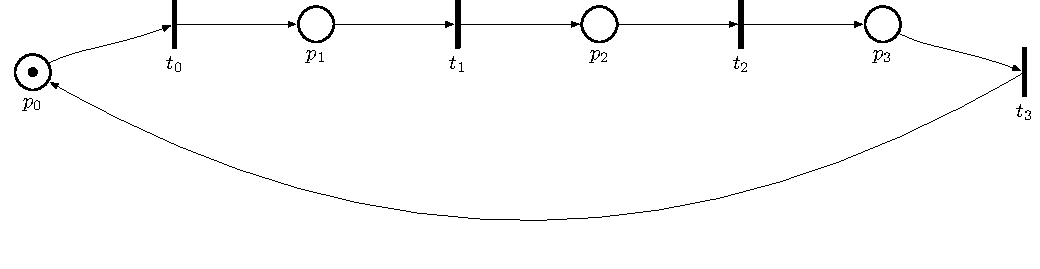
\includegraphics[width=0.8\textwidth]{cipnExample/cipn.tikz}
%   \caption[cipnexample]{Example of Control Interpreted Petri Net to control
%     system in \autoref{fig:cipnexamplescheme}}
%   \label{fig:cipnexample}
% \end{figure}

% \begin{table}[htbp]
\caption{Control Interpreted Petri Net Example Places.}
\centering
\begin{tabular}{M{5cm}M{10cm}}
Places & Meaning\\
\hline
\hyperlink{cipnExampleNet:p0m1}{\hypertarget{cipnExampleTable:p0m1}{$p_{0}$}} & System Stopped\\
\hyperlink{cipnExampleNet:p1}{\hypertarget{cipnExampleTable:p1}{$p_{1}$}} & R (Car Moving to the Right)\\
\hyperlink{cipnExampleNet:p2}{\hypertarget{cipnExampleTable:p2}{$p_{2}$}} & Open (Container Opened)\\
\hyperlink{cipnExampleNet:p3}{\hypertarget{cipnExampleTable:p3}{$p_{3}$}} & L (Car Moving to the Left)\\
\end{tabular}
\end{table}

% \begin{table}[H]
\caption{Control Interpreted Petri Net Example Transitions.}
\centering
\begin{tabular}{M{5cm}M{10cm}}
Transitions & Meaning\\
\hline
\hyperlink{cipnExampleNet:t0}{\hypertarget{cipnExampleTable:t0}{$t_{0}$}} & m (filling request)\\
\hyperlink{cipnExampleNet:t1}{\hypertarget{cipnExampleTable:t1}{$t_{1}$}} & b (Right Limit Switch)\\
\hyperlink{cipnExampleNet:t2}{\hypertarget{cipnExampleTable:t2}{$t_{2}$}} & p (Car is Full)\\
\hyperlink{cipnExampleNet:t3}{\hypertarget{cipnExampleTable:t3}{$t_{3}$}} & a (Left Limit Switch)\\
\end{tabular}
\end{table}

\usetikzlibrary{arrows,shapes,circuits.plc.ladder,external}

\begin{figure}[H]
  \centering
  \includegraphics{cipnExample/cipnLadder.tikz}
  \caption[cipnexample]{Example of Control Interpreted Petri Net converted to Ladder.}
  \label{fig:cipnexampleLadder}
\end{figure}

\begin{figure}[H]
    \centering
    \begin{subfigure}[t]{0.5\textwidth}
        \centering
        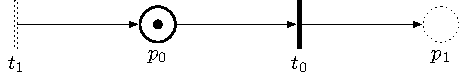
\includegraphics[width=\textwidth]{communicationPlcPN/communicationPlcPN.tikz}
        \caption{Petri Net on PLC 1.}
        \label{fig:communicationPlcPN}
    \end{subfigure}%
    ~ 
    \begin{subfigure}[t]{0.5\textwidth}
        \centering
  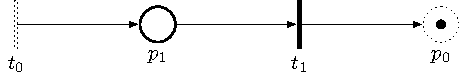
\includegraphics[width=\textwidth]{communicationPlcPN/communicationPlcPN1.tikz}
  \caption{Petri Net on PLC 2.}
  \label{fig:communicationPlcPN1}
    \end{subfigure}
    \caption{Example of Petri Net divided between 2 PLCs.}
\end{figure}


\begin{figure}[H]
    \centering
    \begin{subfigure}[t]{0.45\textwidth}
        \centering
        \includegraphics{communicationPlcPN/communicationPlcPNLadder.tikz}
        \caption{Ladder Logic on PLC 1.}
        \label{fig:communicationPlcPN}
    \end{subfigure}%
\hfill
    \begin{subfigure}[t]{0.45\textwidth}
        \centering
        \includegraphics{communicationPlcPN/communicationPlcPN1Ladder.tikz}
  \caption{Ladder Logic on PLC 2.}
  \label{fig:communicationPlcPN1}
    \end{subfigure}
    \caption{Example of Petri Net divided between 2 PLCs.}
\end{figure}
  

\autoref{fig:communicationPlcPN}






\usetikzlibrary{patterns}
\begin{figure}[H]
  \centering
  \includegraphics[width=0.5\textwidth]{vennDiagramLanguages.tikz}
  \caption{Venn diagram showing relations between $L_{Orig}$, $L_{OrigNI}$,
    $L_{Obs}$, $L_{Exc}$ and $L_{Iden}$}
\end{figure}


%%% Local Variables:
%%% mode: latex
%%% TeX-master: "../monografia.tex"
%%% End: